\documentclass[a4paper, foldmark, notumble]{leaflet}
\usepackage[utf8]{inputenc}
\usepackage[T1]{fontenc}
\usepackage{libertine}
\usepackage{tikz}
\renewcommand*\familydefault{\sfdefault}
\usepackage{lipsum}

\definecolor{primary}{HTML}{6CC24A}
\definecolor{secondary}{HTML}{6E7CA0}
\definecolor{accent}{HTML}{003A70}
\definecolor{alert}{HTML}{DA291C}

\title{Carta de Cores Oficiais do RobSIC}


\AddToBackground{5}{
\begin{tikzpicture}
  \node[shape=rectangle, minimum width=\paperwidth, minimum height=\paperheight] (img) at (0,0) {};
  \node at (2.5,-9) {\includegraphics[width=.3\paperwidth]{png/logo_RobSIC}};
\end{tikzpicture}
}

\begin{document}

\pagestyle{empty}

\section{Cor Secundária}
\begin{center}
  {\large\bfseries Pantone 7667 C}\\
  {\large\bfseries HEX \#6E7CA0}
  \vskip3mm
  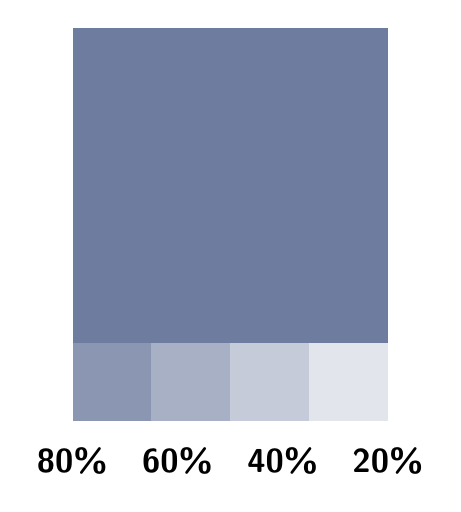
\begin{tikzpicture}
    \fill [secondary] (0,0) rectangle (4,5);
    \fill [secondary!80] (0,0) rectangle (1,1);
    \fill [secondary!60] (1,0) rectangle (2,1);
    \fill [secondary!40] (2,0) rectangle (3,1);
    \fill [secondary!20] (3,0) rectangle (4,1);
    \node at (2,-.5) {\large\bfseries 80\% \; 60\% \; 40\% \; 20\%};
  \end{tikzpicture}
\end{center}

\begin{center}
  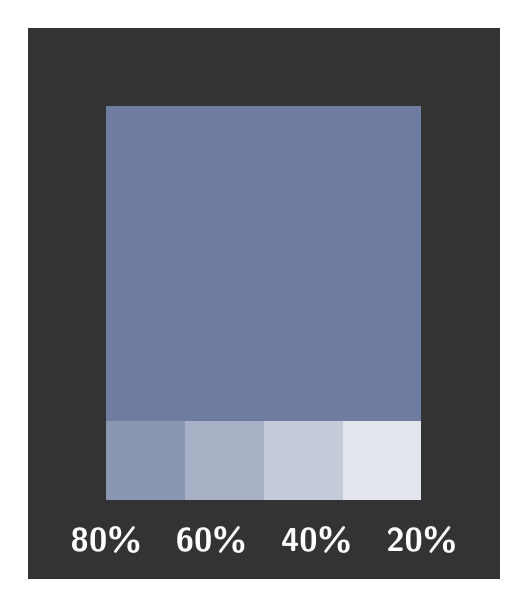
\begin{tikzpicture}
    \fill [black!80] (-1,-1) rectangle (5,6);
    \fill [secondary] (0,0) rectangle (4,5);
    \fill [secondary!80] (0,0) rectangle (1,1);
    \fill [secondary!60] (1,0) rectangle (2,1);
    \fill [secondary!40] (2,0) rectangle (3,1);
    \fill [secondary!20] (3,0) rectangle (4,1);
    \node[text=white] at (2,-.5) {\large\bfseries 80\% \; 60\% \; 40\% \; 20\%};
  \end{tikzpicture}
\end{center}
\pagebreak

\section{Cor de Destaque}
\begin{center}
  {\large\bfseries Pantone 654}\\
  {\large\bfseries HEX \#003A70}
    \vskip3mm
  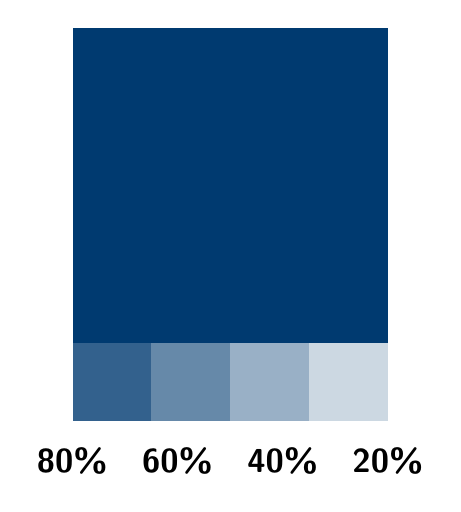
\begin{tikzpicture}
    \fill [accent] (0,0) rectangle (4,5);
    \fill [accent!80] (0,0) rectangle (1,1);
    \fill [accent!60] (1,0) rectangle (2,1);
    \fill [accent!40] (2,0) rectangle (3,1);
    \fill [accent!20] (3,0) rectangle (4,1);
    \node at (2,-.5) {\large\bfseries 80\% \; 60\% \; 40\% \; 20\%};
  \end{tikzpicture}
\end{center}

\begin{center}
  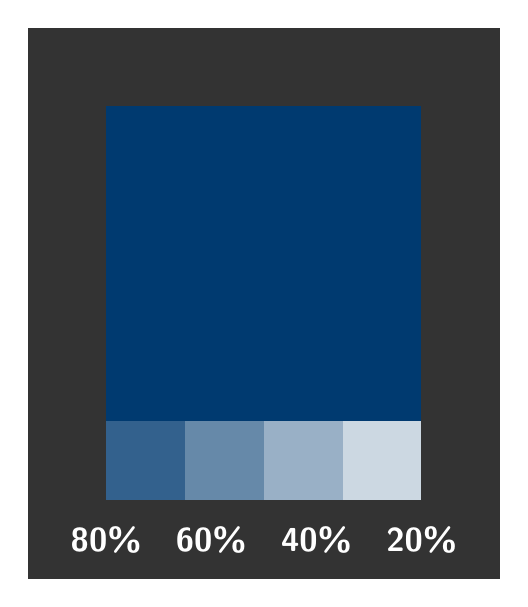
\begin{tikzpicture}
    \fill [black!80] (-1,-1) rectangle (5,6);
    \fill [accent] (0,0) rectangle (4,5);
    \fill [accent!80] (0,0) rectangle (1,1);
    \fill [accent!60] (1,0) rectangle (2,1);
    \fill [accent!40] (2,0) rectangle (3,1);
    \fill [accent!20] (3,0) rectangle (4,1);
    \node[text=white] at (2,-.5) {\large\bfseries 80\% \; 60\% \; 40\% \; 20\%};
  \end{tikzpicture}
\end{center}

\pagebreak

\section{Cor de Alerta}
\begin{center}
  {\large\bfseries Pantone 485}\\
  {\large\bfseries HEX \#DA291C}
  \vskip3mm
  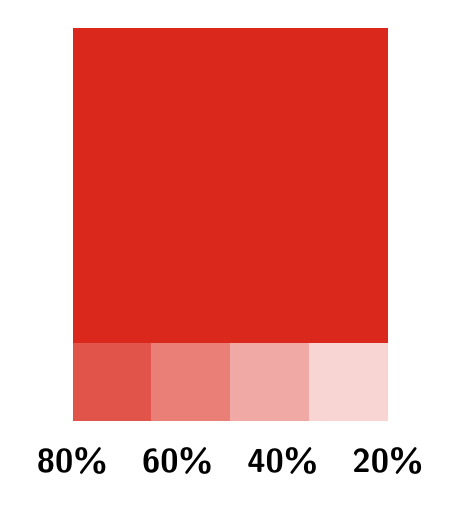
\begin{tikzpicture}
    \fill [alert] (0,0) rectangle (4,5);
    \fill [alert!80] (0,0) rectangle (1,1);
    \fill [alert!60] (1,0) rectangle (2,1);
    \fill [alert!40] (2,0) rectangle (3,1);
    \fill [alert!20] (3,0) rectangle (4,1);
    \node at (2,-.5) {\large\bfseries 80\% \; 60\% \; 40\% \; 20\%};
  \end{tikzpicture}
\end{center}

\begin{center}
  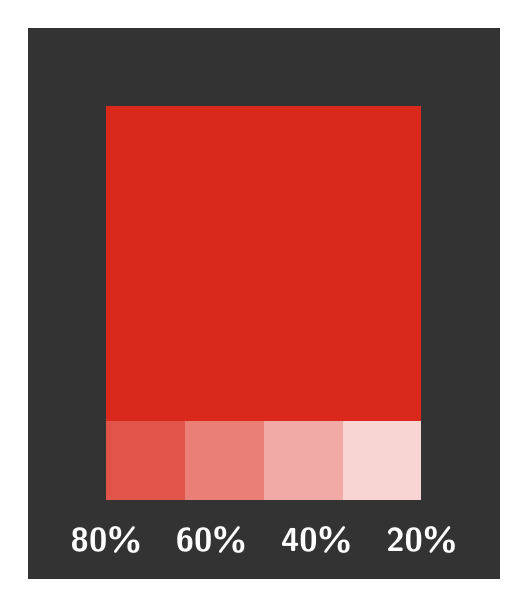
\begin{tikzpicture}
    \fill [black!80] (-1,-1) rectangle (5,6);
    \fill [alert] (0,0) rectangle (4,5);
    \fill [alert!80] (0,0) rectangle (1,1);
    \fill [alert!60] (1,0) rectangle (2,1);
    \fill [alert!40] (2,0) rectangle (3,1);
    \fill [alert!20] (3,0) rectangle (4,1);
    \node[text=white] at (2,-.5) {\large\bfseries 80\% \; 60\% \; 40\% \; 20\%};
  \end{tikzpicture}
\end{center}

\pagebreak

\section{Logos}

\pagebreak


\maketitle
\thispagestyle{empty}

\lipsum[1-2]

\pagebreak

\section{Cor Principal}

\begin{center}
  {\large\bfseries Pantone 360 C}\\
  {\large\bfseries HEX \#6CC24A}\\
  \vskip3mm
  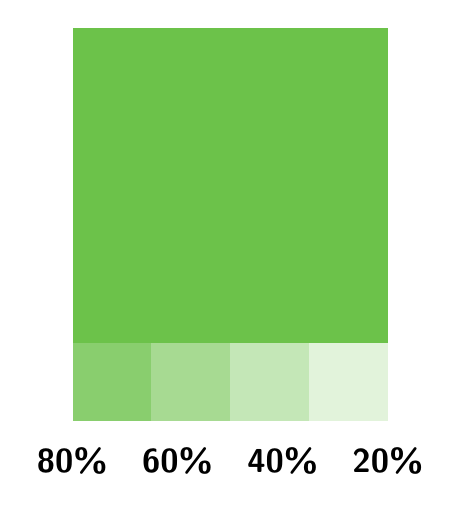
\begin{tikzpicture}
    \fill [primary] (0,0) rectangle (4,5);
    \fill [primary!80] (0,0) rectangle (1,1);
    \fill [primary!60] (1,0) rectangle (2,1);
    \fill [primary!40] (2,0) rectangle (3,1);
    \fill [primary!20] (3,0) rectangle (4,1);
    \node at (2,-.5) {\large\bfseries 80\% \; 60\% \; 40\% \; 20\%};
  \end{tikzpicture}
\end{center}

\begin{center}
  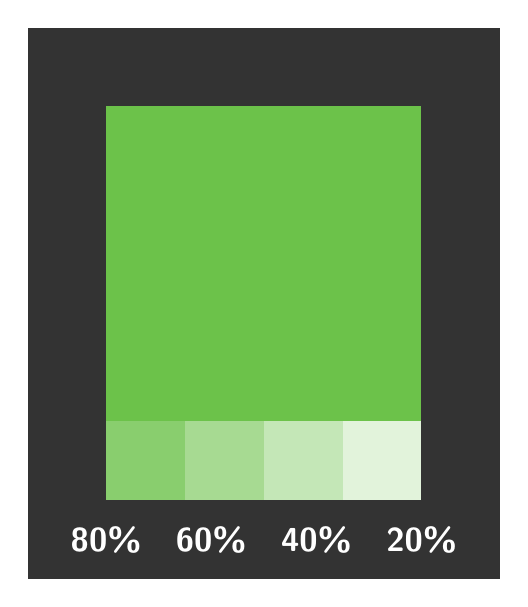
\begin{tikzpicture}
    \fill [black!80] (-1,-1) rectangle (5,6);
    \fill [primary] (0,0) rectangle (4,5);
    \fill [primary!80] (0,0) rectangle (1,1);
    \fill [primary!60] (1,0) rectangle (2,1);
    \fill [primary!40] (2,0) rectangle (3,1);
    \fill [primary!20] (3,0) rectangle (4,1);
    \node[text=white] at (2,-.5) {\large\bfseries 80\% \; 60\% \; 40\% \; 20\%};
  \end{tikzpicture}
\end{center}

\end{document}
